\chapter{Time Evolution Algorithm}

In order to efficiently perform the time evolution a slightly modified version of the TEBD algorithm was employed. Since the Hamiltonian is changing with every time step, one has to account for the time spent exponentiating the operators when considering the runtime of the algorithm. For a general operator $\hat{W}$ this can be achieved through the series expansion
\begin{equation}
	\exp \left( \hat{W} \right) = \sum_{k = 0}^{\infty} \frac{\hat{W}^k}{k!} = \hat{\mathds{1}} + \hat{W} \Bigl(  \hat{\mathds{1}} + \frac{\hat{W}}{2} \Bigl( \hat{\mathds{1}} + \frac{\hat{W}}{3} \Bigl( \ldots
\end{equation}
The number of terms needed in the expansion to accurately describe the exponentiation depends on the operator. As the cost of exponentiating the hopping terms of the Bose-Hubbard Hamiltonian was relatively high, it was concluded that keeping $J$ fixed and using $U$ as the control parameter was the better option. Hence, only the terms $\frac{U}{2} \hat{n}_i (\hat{n}_i -1)$ had to be exponentiated at every time step, which could be done fairly quickly due the diagonal form of the operator. However, in order to be able to consider the tunnelling and interaction contributions to the time evolution separately, one most expand the time evolution operator into its components. By employing the Suzuki-Trotter expansion the otherwise single tensor of the time evolution operator can be decomposed into separate tensors for each term of the Hamiltonian. To second order this expansion read
\begin{equation}
	\exp\left(  ( \hat{V} + \hat{W}  ) \delta \right) = \exp\left(  \hat{V} \delta /2  \right) \exp\left(  \hat{W} \delta   \right) \exp\left(  \hat{V} \delta /2  \right) + O(\delta^3) \; . \label{eq:SuzukiTrotter}
\end{equation}
Thus, one can divide the time evolution operator into a sequence of tensors, where
\begin{align}
	\hat{\mathcal{U}}_{J}^{[i,i+1]} (\delta t/2) &= \exp \left( -i J ( \hat{a}_{i}^{\dag} \hat{a}_{i+1} + \hat{a}_{i+1}^{\dag} \hat{a}_{i} ) \frac{\delta t}{2} / \hbar \right) \\
	\hat{\mathcal{U}}_{U}^{[i]} (\delta t) &= \exp \left( -i \frac{U}{2} \hat{n}_i (\hat{n}_i -1) \delta t / \hbar \right) \; .
\end{align}
\begin{figure}[h!]
	\centering
	\begin{tikzpicture}[inner sep=1mm]
\def \reldist {2};
\def \numb {4};
\def \wid {3.2};
\def \size {1.0};
\def \hi {0.8};
\def \vert {1.0};
\def \rad {0.4};

	
\foreach \i in  {1,...,\numb} {
	\node[tensor,minimum width= \size cm,minimum height= \size cm, rounded corners = 0.2cm] (A\i)
	at (\i * \reldist, 0) {$A^{[ \i ]}$};
	\draw[-] (A\i) -- (\i * \reldist , -\numb*\vert -1.8);	
};

\foreach \i in {1,...,3} {
    \pgfmathtruncatemacro{\iplusone}{\i + 1};
    \draw[-] (A\i) -- (A\iplusone);
};

\foreach \i in {1,...,\numb} {
	\pgfmathtruncatemacro{\j}{\i + 1};
    \node[twositeop, minimum width= \wid cm,minimum height= \hi cm,rounded corners = \rad cm] (fop\i)
    at (\reldist*\i + \reldist/2, -\vert*\i -0.1)
    {\small $\hat{\mathcal{U}}_{J}^{[ \i , \j ]} (\delta t /2)$};
};
	
	
\foreach \i in  {1,...,\numb} {
	\node[operator,minimum width= \hi cm,minimum height= \hi cm] (op\i)
	at (\i * \reldist, -\vert*\i -0.1 - \vert)
	{\scriptsize $\hat{\mathcal{U}}_{U}^{[ \i ]}$};	
};


\foreach \i in  {1,...,\numb} {
	\node (dots\i) at (\i * \reldist, -\numb*\vert -2) {\normalsize $\vdots$};
	\draw[-] (dots\i) -- (\i * \reldist , -2*\numb*\vert -2.7);	
};

\foreach \i in {1,...,\numb} {
	\pgfmathtruncatemacro{\j}{\i + 1};
    \node[twositeop, minimum width= \wid cm,minimum height= \hi cm,rounded corners = \rad cm] (sop\i)
    at (\reldist*\i + \reldist/2, \vert*\i -2*\numb*\vert - 3)
    {\small $\hat{\mathcal{U}}_{J}^{[ \i , \j ]} (\delta t /2)$};
};



\draw[decoration={calligraphic brace,amplitude=10pt}, decorate, line width=1.25pt, xshift=-4pt, yshift=0pt]
(0, -2*\numb*\vert -2.5) -- (0,-0.8) node [black,midway,xshift=-0.6cm] 
{\large $\delta t$};


	\node (dot2) at (\numb * \reldist + 2.4,0) {$\dots$};

	\draw[-] (A\numb) -- (dot2);
	
	
\end{tikzpicture}
	\caption{\textit{Tensor diagram depicting a single time step of the modified TEBD algorithm. The time evolution operator has been subjected to a Suzuki-Trotter expansion as detailed in eq. \eqref{eq:SuzukiTrotter}. The tensors of the upper part of the network are contracted with the MPS while sweeping from left to right, whereas the lower part is applied with a right to left sweep.}}
	\label{fig:ModifiedTEBD}
\end{figure}
A single time step, $\delta t$, using the expanded operator is represented diagrammatically in figure \ref{fig:ModifiedTEBD}. At first glance, the tensor network resulting from the Suzuki-Trotter expansion may seem too extensive, however, it can be contracted in a very efficient manner. The upper part of the network is contracted in a left to right sweeping manner, where one following each contraction pushes the position of the center cite, and thereby the normalisation, of the MPS to the right.
\begin{figure}
\centering % <-- add this
\begin{subfigure}[b]{0.35\textwidth}
	\caption{}  
  	\begin{tikzpicture}[inner sep=1mm]
\def \reldist {2};
\def \numb {4};
\def \wid {3.2};
\def \size {1.0};
\def \rad {0.5};



\node[tensorc,minimum width= \size cm,minimum height= \size cm, rounded corners = 0.2cm] (A1) at (1 * \reldist, 0) {$A^{[1]}$};

\node[tensorr,minimum width= \size cm,minimum height= \size cm, rounded corners = 0.2cm] (A2) at (2 * \reldist, 0) {$A^{[2]}$};

\node[tensorr,minimum width= \size cm,minimum height= \size cm, rounded corners = 0.2cm] (A3) at (3 * \reldist, 0) {$A^{[3]}$};

\node[tensorr,minimum width= \size cm,minimum height= \size cm, rounded corners = 0.2cm] (A4) at (4 * \reldist, 0) {$A^{[4]}$};

\foreach \i in  {1,...,\numb} {
	\draw[-] (A\i) -- (\i * \reldist , -8.5);	
};

\foreach \i in {1,...,3} {
    \pgfmathtruncatemacro{\iplusone}{\i + 1};
    \draw[-] (A\i) -- (A\iplusone);
};

\node[twositeop, minimum width= \wid cm,minimum height= \size cm,rounded corners = \rad cm] (fop1)
    at (\reldist*1 + \reldist/2,-1.5)
    {\small $\hat{\mathcal{U}}_{J}^{[1,2]}(\delta t /2)$};
    
\node[twositeop, minimum width= \wid cm,minimum height= \size cm,rounded corners = \rad cm] (fop3)
    at (\reldist*3 + \reldist/2,-1.5)
    {\small $\hat{\mathcal{U}}_{J}^{[3,4]}(\delta t /2)$};

\node[twositeop, minimum width= \wid cm,minimum height= \size cm,rounded corners = \rad cm] (fop2)
    at (\reldist*2 + \reldist/2,-3)
    {$\hat{\mathcal{U}}_{J}^{[2,3]}(\delta t /2)$};
	
	
\foreach \i in  {1,...,\numb} {
	\node[operator,minimum width= \size cm,minimum height= \size cm] (op\i)
	at (\i * \reldist, -4.5)
	{\scriptsize $\hat{\mathcal{U}}_{U}(\delta t)$};	
};

\node[twositeop, minimum width= \wid cm,minimum height= \size cm,rounded corners = \rad cm] (sop1)
    at (\reldist*1 + \reldist/2,-6)
    {\small $\hat{\mathcal{U}}_{J}^{[1,2]}(\delta t /2)$};
    
\node[twositeop, minimum width= \wid cm,minimum height= \size cm,rounded corners = \rad cm] (sop3)
    at (\reldist*3 + \reldist/2,-6)
    {\small $\hat{\mathcal{U}}_{J}^{[3,4]}(\delta t /2)$};

\node[twositeop, minimum width= \wid cm,minimum height= \size cm,rounded corners = \rad cm] (sop2)
    at (\reldist*2 + \reldist/2,-7.5)
    {$\hat{\mathcal{U}}_{J}^{[2,3]}(\delta t /2)$};



	\node (dot2) at (\numb * \reldist + 2.4,0) {$\dots$};
	\draw[-] (A\numb) -- (dot2);
	
	
\end{tikzpicture}
\end{subfigure}
\begin{subfigure}[b]{0.35\textwidth}
	\caption{}    
  	\begin{tikzpicture}[inner sep=1mm]
\def \reldist {2};
\def \numb {4};
\def \wid {3.2};
\def \size {1.0};
\def \rad {0.5};



\node[tensorc,minimum width= \size cm,minimum height= \size cm, rounded corners = 0.2cm] (A1) at (1 * \reldist, 0) {$A^{[1]}$};

\node[tensorr,minimum width= \size cm,minimum height= \size cm, rounded corners = 0.2cm] (A2) at (2 * \reldist, 0) {$A^{[2]}$};

\node[tensorr,minimum width= \size cm,minimum height= \size cm, rounded corners = 0.2cm] (A3) at (3 * \reldist, 0) {$A^{[3]}$};

\node[tensorr,minimum width= \size cm,minimum height= \size cm, rounded corners = 0.2cm] (A4) at (4 * \reldist, 0) {$A^{[4]}$};

\node[tensor,minimum width= \wid cm,minimum height= \size cm, rounded corners = 0.2cm] (AA) at (\reldist*1 + \reldist/2, 0) {$\Theta$};

\foreach \i in  {1,...,\numb} {
	\draw[-] (A\i) -- (\i * \reldist , -8.5);	
};

\foreach \i in {1,...,3} {
    \pgfmathtruncatemacro{\iplusone}{\i + 1};
    \draw[-] (A\i) -- (A\iplusone);
};

\node[twositeop, minimum width= \wid cm,minimum height= \size cm,rounded corners = \rad cm] (fop1)
    at (\reldist*1 + \reldist/2,-1.5)
    {\small $\hat{\mathcal{U}}_{J}^{[1,2]}(\delta t /2)$};
    
\node[twositeop, minimum width= \wid cm,minimum height= \size cm,rounded corners = \rad cm] (fop3)
    at (\reldist*3 + \reldist/2,-1.5)
    {\small $\hat{\mathcal{U}}_{J}^{[3,4]}(\delta t /2)$};

\node[twositeop, minimum width= \wid cm,minimum height= \size cm,rounded corners = \rad cm] (fop2)
    at (\reldist*2 + \reldist/2,-3)
    {$\hat{\mathcal{U}}_{J}^{[2,3]}(\delta t /2)$};
	
	
\foreach \i in  {1,...,\numb} {
	\node[operator,minimum width= \size cm,minimum height= \size cm] (op\i)
	at (\i * \reldist, -4.5)
	{\scriptsize $\hat{\mathcal{U}}_{U}(\delta t)$};	
};

\node[twositeop, minimum width= \wid cm,minimum height= \size cm,rounded corners = \rad cm] (sop1)
    at (\reldist*1 + \reldist/2,-6)
    {\small $\hat{\mathcal{U}}_{J}^{[1,2]}(\delta t /2)$};
    
\node[twositeop, minimum width= \wid cm,minimum height= \size cm,rounded corners = \rad cm] (sop3)
    at (\reldist*3 + \reldist/2,-6)
    {\small $\hat{\mathcal{U}}_{J}^{[3,4]}(\delta t /2)$};

\node[twositeop, minimum width= \wid cm,minimum height= \size cm,rounded corners = \rad cm] (sop2)
    at (\reldist*2 + \reldist/2,-7.5)
    {$\hat{\mathcal{U}}_{J}^{[2,3]}(\delta t /2)$};



	\node (dot2) at (\numb * \reldist + 2.4,0) {$\dots$};
	\draw[-] (A\numb) -- (dot2);
	
	
\end{tikzpicture}
\end{subfigure}
\\ % <-- add this
\vspace{10mm}
\begin{subfigure}[b]{0.35\textwidth}
	\caption{}    	
  	\begin{tikzpicture}[inner sep=1mm]
\def \reldist {2};
\def \numb {2};
\def \wid {3.2};
\def \size {1.0};
\def \rad {0.5};



\node[tensor,minimum width= \size cm,minimum height= \size cm, rounded corners = 0.2cm] (A1) at (1 * \reldist, 0) {$A^{[1]}$};

\node[tensor,minimum width= \size cm,minimum height= \size cm, rounded corners = 0.2cm] (A2) at (2 * \reldist, 0) {$A^{[2]}$};


\foreach \i in  {1,...,\numb} {
	\draw[-] (A\i) -- (\i * \reldist ,-2.5);	
};
   
\draw[-] (A1) -- (A2);    

\node[twositeop, minimum width= \wid cm,minimum height= \size cm,rounded corners = \rad cm] (fop2)
    at (\reldist*2 + \reldist/2, -1.5 )
    {$\hat{\mathcal{U}}_{J}^{[2,3]}(\delta t /2)$};
	
\node[operator,minimum width= \size cm,minimum height= \size cm] (op1)
	at ( \reldist, -1.5)
	{\scriptsize $\hat{\mathcal{U}}_{U}(\delta t)$};	

\draw[-,line width=0.8mm] (A1) -- (op1);

\node (dot2) at (\numb * \reldist + 1.4,0) {$\dots$};
\draw[-] (A\numb) -- (dot2);
	
	
\end{tikzpicture}
\end{subfigure}
\begin{subfigure}[b]{0.35\textwidth}
	\caption{}  
  	\begin{tikzpicture}[inner sep=1mm]
\def \reldist {1.5};
\def \numb {4};
\def \wid {2.3};
\def \size {1.0};
\def \hi {0.8};
\def \rad {0.4};
\def \vert {1.35};


\foreach \i in  {1,...,\numb} {
	\node[tensorr,minimum width= \size cm,minimum height= \size cm, rounded corners = 0.2cm] (A\i)
	at (\i * \reldist, 0) {$M^{[ \i ]}$};
	\draw[-] (A\i) -- (\i * \reldist , -2.5*\vert);	
};

\foreach \i in {1,...,3} {
    \pgfmathtruncatemacro{\iplusone}{\i + 1};
    \draw[-] (A\i) -- (A\iplusone);
};

\node[tensorl,minimum width= \size cm,minimum height= \size cm, rounded corners = 0.2cm] (L1) at (1 * \reldist, 0) {$M^{[1]}$};

\node[tensorl,minimum width= \size cm,minimum height= \size cm, rounded corners = 0.2cm] (L2) at (2 * \reldist, 0) {$M^{[2]}$};

\node[tensorc,minimum width= \size cm,minimum height= \size cm, rounded corners = 0.2cm] (C) at (3 * \reldist, 0) {$M^{[3]}$};


\foreach \i in  {1,...,\numb} {
	\draw[-] (A\i) -- (\i * \reldist , -2.6 *\vert);	
};

\draw[-,line width=0.8mm] (A3) -- (A4);

\foreach \i in  {3,...,\numb} {
	\node[operator,minimum width= \hi cm,minimum height= \hi cm] (op\i)
	at (\i * \reldist, -\vert)
	{\scriptsize $\hat{\mathcal{U}}_{U}^{[ \i ]}$};	
};

\foreach \i in {3} {
	\pgfmathtruncatemacro{\j}{\i + 1};
    \node[twositeop, minimum width= \wid cm,minimum height= \hi cm,rounded corners = \rad cm] (top\i)
    at (\reldist*\i + \reldist/2, -2*\vert)
    {\small $\hat{\mathcal{U}}_{J}^{[ \i , \j ]} $};
};


\node (dot2) at (\numb * \reldist + 1.4,0) {$\dots$};
\draw[-] (A\numb) -- (dot2);
	
	
\end{tikzpicture}
\end{subfigure}
\caption{\textit{Sequence of contractions for modified TEBD algorithm during left to right sweep. Step \textbf{(i)}: MPS centred on site 1, tensors $A^{[1]}$ and $A^{[2]}$ are contracted. Step \textbf{(ii)}: Two-site tensor is contracted with two-site operator, followed by a splitting of the resulting tensor through an SVD in step \textbf{(iii)}. Lastly, in step \textbf{(iv)}, the center (and thereby the normalisation) is pushed to the next site leaving $A^{[1]}$ left-normalised.}}
\label{fig:TEBDContraction}
\end{figure}
An example of this is shown in figure \ref{fig:TEBDContraction}. The MPS is initially centred on the first tensor, while its remaining tensors are all right-normalised. By following the depicted sequence of contractions marked with bold lines, the operators are efficiently applied to the MPS. In step (iii) the two-site tensor, $\Theta$, is split using an SVD, where the bond dimension of the tensors are truncated. This is crucial in order to maintain a reduced dimensionality, which would otherwise result in a significant increase in contraction time. In the last step the MPS is centred on the next site leaving the previous center left-normalised. Thereby the normalisation of the MPS is "pushed" to the right and contained in a single site, which makes it easy to deal with in the end of the time evolution step.
As the centre reaches the end of the MPS, the direction of the sweep is reversed. The right to left sweep is slightly different, as there are no $\hat{\mathcal{U}}_{U}$-tensors that need to be contracted. The time evolution step is completed, as the first site is reached. 


\begin{figure}[h]
	\centering
	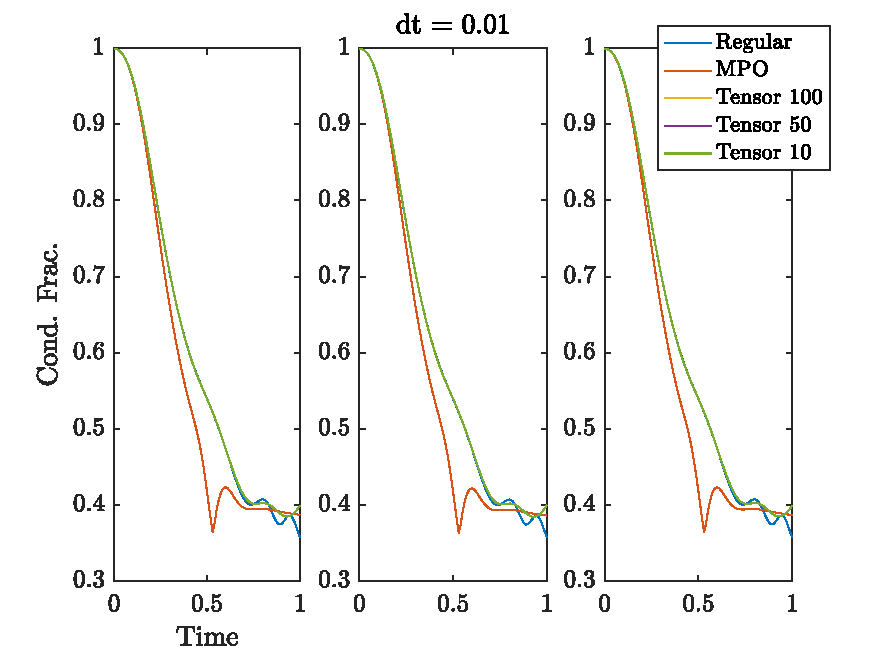
\includegraphics[width=0.9\textwidth]{Figures/TimeEvolve1.pdf}
	\caption{\textit{}}
	\label{fig:TimeEvolve1}
\end{figure}

\begin{figure}[h]
	\centering
	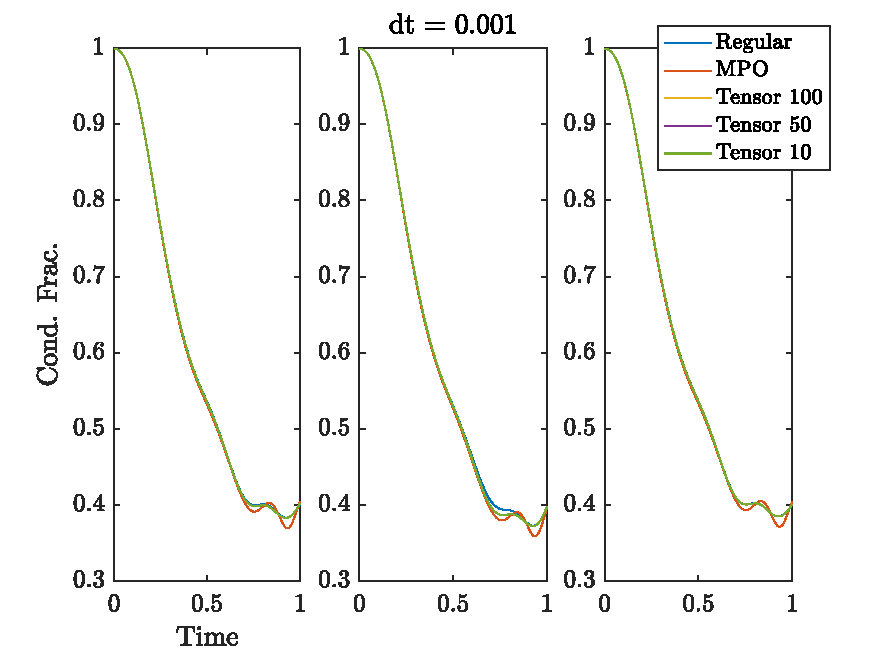
\includegraphics[width=0.9\textwidth]{Figures/TimeEvolve2.pdf}
	\caption{\textit{}}
	\label{fig:TimeEvolve2}
\end{figure}

\begin{figure}[h]
	\centering
	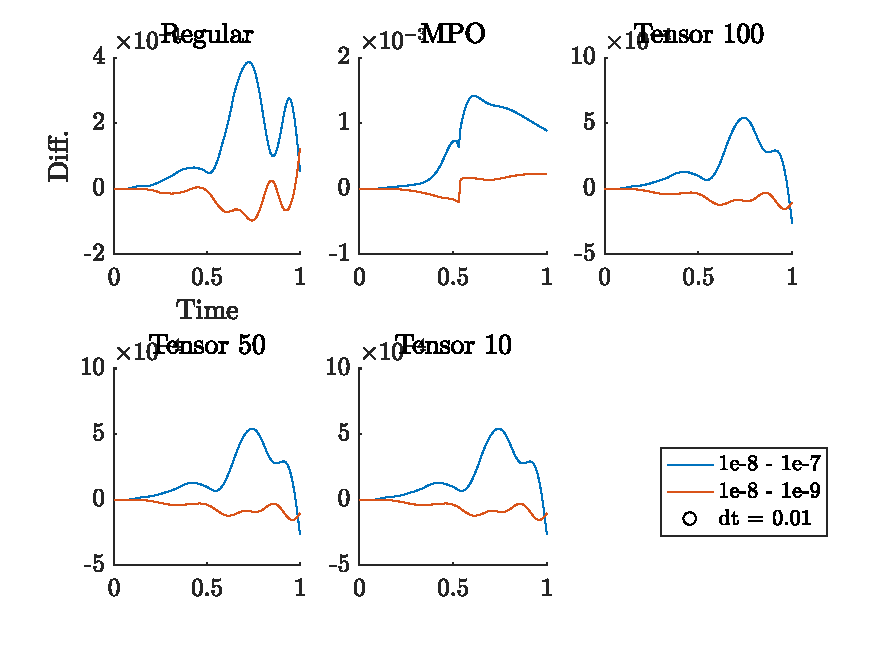
\includegraphics[width=0.9\textwidth]{Figures/CompareCutoffs1.pdf}
	\caption{\textit{}}
	\label{fig:Cutoff1}
\end{figure}

\begin{figure}[h]
	\centering
	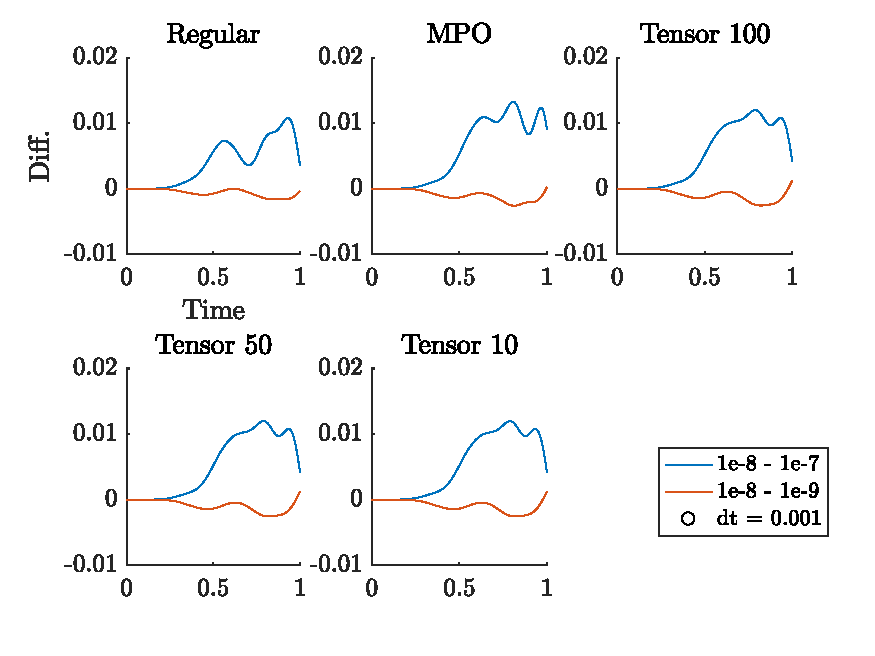
\includegraphics[width=0.9\textwidth]{Figures/CompareCutoffs2.pdf}
	\caption{\textit{}}
	\label{fig:Cutoff2}
\end{figure}

\begin{figure}[h]
	\centering
	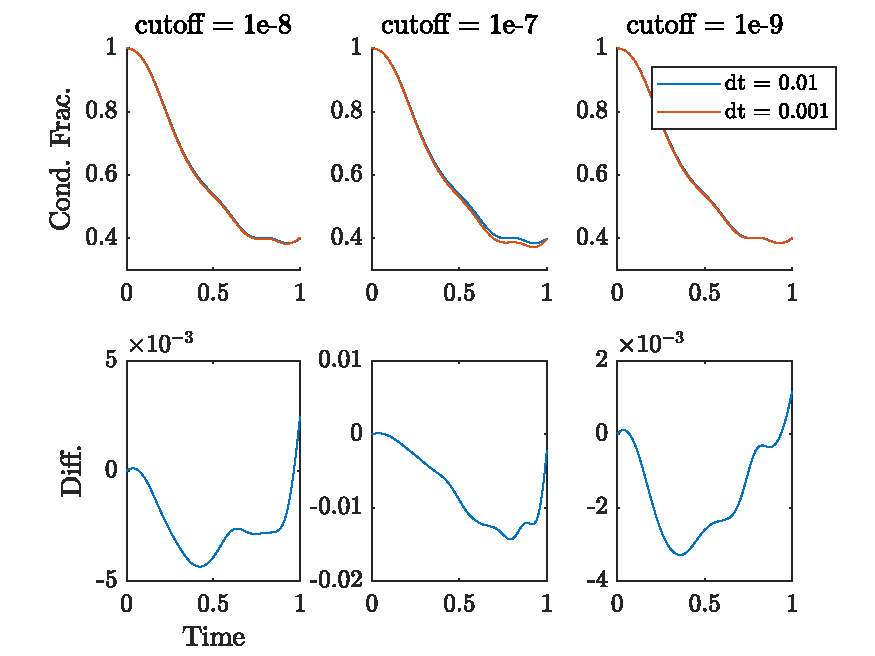
\includegraphics[width=0.9\textwidth]{Figures/CompareTimeStep.pdf}
	\caption{\textit{}}
	\label{fig:TimeStep}
\end{figure}

\end{document}